\documentclass[10pt,aspectratio=169]{beamer}
% For Chinese text, uncomment this line and compile with XeLaTeX:
% \usepackage[UTF8,fontset=fandol]{ctex}
\usepackage{dku}

% Short forms in brackets appear in the footer.
\title{Duke Kunshan University}
\subtitle{Beamer Presentation Theme}
\author[Your Name]{Your Name}
\institute[DKU]{Your Department}
\date{\today}

\lstset{basicstyle=\ttfamily\footnotesize,frame=single,language=Python}

\begin{document}
\maketitle

\section{Getting Started}

\begin{frame}{Getting Started}
  \begin{itemize}
    \item Edit the title, author, department and date in \texttt{main.tex}.
    \item Add content using standard Beamer frames.
    \item Compile with XeLaTeX; theme settings are in \texttt{dku.sty}.
  \end{itemize}
  \begin{block}{About this theme}
    An unofficial Duke Kunshan University theme for academic presentations.
  \end{block}
\end{frame}

\begin{frame}[fragile]{Presentation Metadata}
\begin{lstlisting}[language=TeX]
\title{Your Presentation Title}
\subtitle{Your Subtitle}
\author[Short Name]{Full Author Name}
\institute[DKU]{Your Department}
\date[Nov. 2026]{November 15, 2026}
\end{lstlisting}
  Optional short forms keep the footer concise.
\end{frame}

\section{Examples}

\begin{frame}{Text and Mathematics}{Clear structure, readable equations}
  \begin{itemize}
    \item Use \textbf{bold} for key terms and \alert{color} for emphasis.
    \item Use \texttt{itemize[<+->]} to reveal items one at a time.
  \end{itemize}
  \begin{equation*}
    \mathrm{i}\hslash\frac{\partial}{\partial t}\Psi(\mathbf{r},t)
    = -\frac{\hslash^2}{2m}\nabla^2\Psi(\mathbf{r},t)
      + V(\mathbf{r})\Psi(\mathbf{r},t).
  \end{equation*}
\end{frame}

\begin{frame}{Columns and Blocks}
  \begin{columns}[T,onlytextwidth]
    \begin{column}{0.48\textwidth}
      \begin{block}{Research Question}
        State the problem and explain why it matters.
      \end{block}
      \begin{itemize}
        \item Background
        \item Approach
      \end{itemize}
    \end{column}
    \begin{column}{0.48\textwidth}
      \begin{exampleblock}{Key Finding}
        Present the main result and its implications.
      \end{exampleblock}
      \begin{itemize}
        \item Evidence
        \item Interpretation
      \end{itemize}
    \end{column}
  \end{columns}
\end{frame}

\begin{frame}{Figures}
  \begin{figure}
    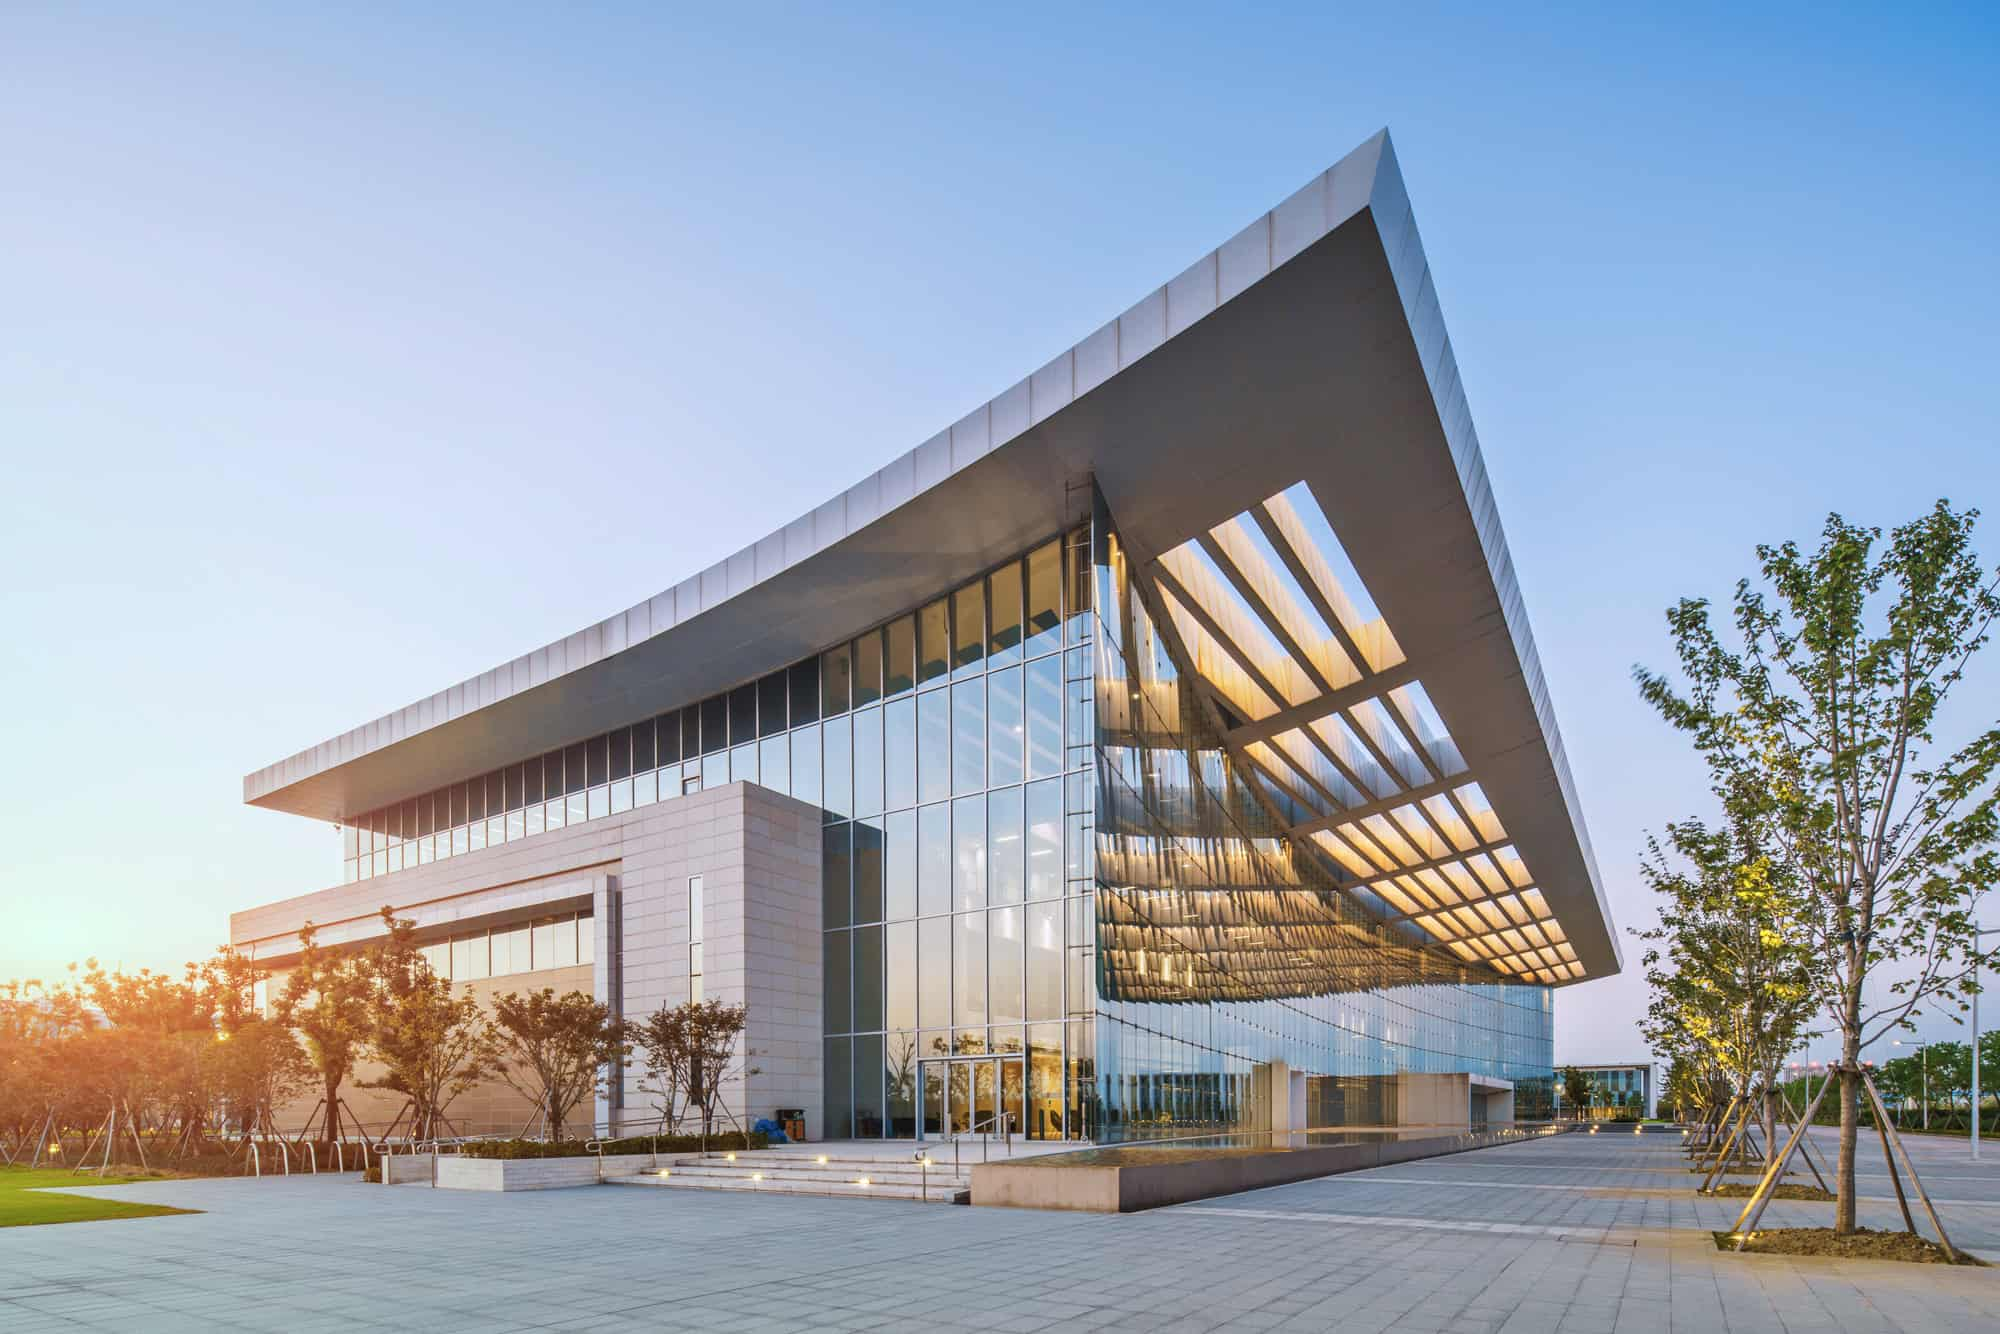
\includegraphics[width=0.46\textwidth]{source/dku/ab-1.jpg}
    \caption{Academic Building, Duke Kunshan University}
  \end{figure}
  {\tiny Source: \href{https://www.dukekunshan.edu.cn/photo-gallery/}{Duke Kunshan University Photo Gallery}.}
\end{frame}

\begin{frame}[fragile]{Code}
\begin{lstlisting}
def fibonacci(n):
    a, b = 0, 1
    for _ in range(n):
        a, b = b, a + b
    return a
\end{lstlisting}
\end{frame}

% Optional custom closing text: \backmatter[Questions?]
\backmatter
\end{document}
